\chapter{Related Work}
\label{ch:related_work}
Many approaches have been proposed to help with deploying DNN on mobile device, either in algorithm or hardward aspect. In this chapter, we will discuss more about the main optimization scheme we choose, which is quantisation, and then existing hardware-designed DNN accelerators.
\section{Quantization}
Quantization maps data to a smaller set of quantization levels. The principle is to minimize the error between the reconstructed data from the quantized one and the original data. The quantization level essentially reflects the bits required to represent the data. Reduced data bits comes with several benefits includes reduced storage costs, memory transactions and computational cost. There are ways to quantization, from simplest uniform distance between each quantization \figref{quant_types}(a) level to special mapping function such as \textit{log} function so that distance between quantization steps are of logarithm relation \figref{quant_types}(b); and even more advanced approaches like clustering data into groups with k-means, requiring look up table for the mapping and computation \figref{quant_types}(c). The simplest quantization also known as \textit{linear quantization} related closely to this project, and we're going to focus on it particularly.
\begin{figure}
    \centering
    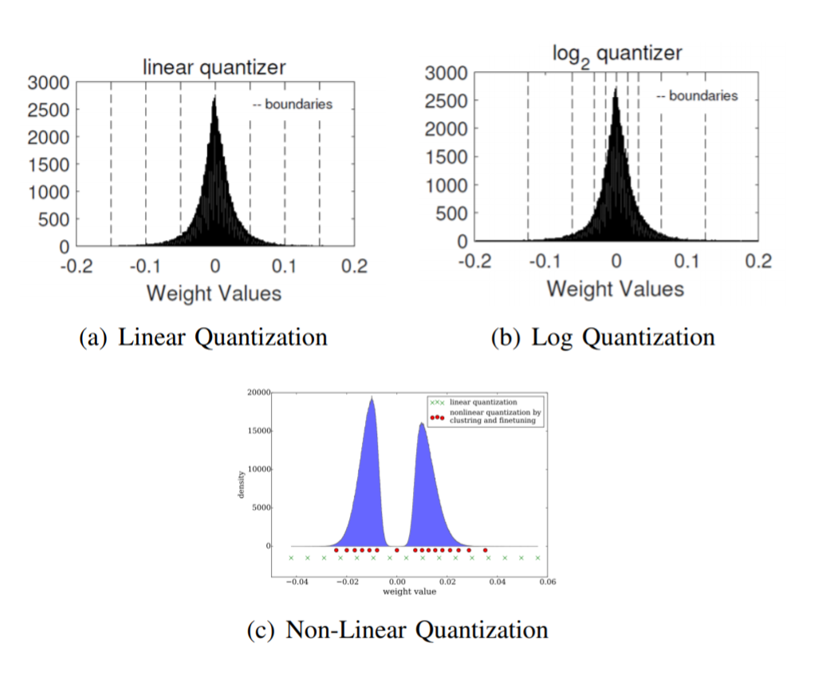
\includegraphics[width=0.8\linewidth]{inc/2_related_work/figure/quantization_types.png}
    \caption{Various methods of quantization from \cite{lognet}\cite{DeepCompression}}
    \label{fig:quant_types}
\end{figure}
\subsection{fixed point quantisation}
More related to this work, researches find the numerical requirement for even the latest DNN model inference stage far from the commonly used 32/64 bit floating-point format. \cite{FixedPoint} quantize the models to fixed point with ${L_2}$ error minimization, achieved \textbf{0.89\%} MCR (miss classification rate) on \textbf{MNIST} with 5 bits weights in comparison to \textbf{0.81\%} MCR with floating point weights.
\subsection{ternary to binary quantisation}
Some researchers have tried extreme quantization down to 2bits tenary weights such as in TWNs\cite{Ternary} and even binary weights in BinaryNet \cite{BinaryNet}, to binarize both weight and activation as in XNOR-net\cite{XnorNet}. \\
TWNs minimizes the Euclidian distance between the full precision weights $\boldsymbol{W}$ and tenary-valued weights $\boldsymbol{W^t}$ along with a non-negative scaling factor $\alpha$ in \eqref{eq:twn} achieving \textbf{99.35\%}, \textbf{92.56\%}, \textbf{84.2\%} on \textbf{MNIST}, \textbf{CIFAR-10}, \textbf{ImageNet(top-5)} dataset respectively.  
\begin{equation}
\begin{aligned}\label{eq:twn}
    \alpha^*, \boldsymbol{W^{t*}} = \mathop{\arg\min}_{\alpha,\boldsymbol{W^t}} = \|\boldsymbol{W}-\alpha\boldsymbol{W^t}\|^2_2 \\  
\text{s.t }\alpha\geq0,\boldsymbol{W^t_i}\in\{1,0,-1\}, i=1,2,...,n.
\end{aligned}
\end{equation}
BinaryNet constrains both weights and activations to either +1 or -1 with 
\begin{equation}
    \begin{aligned}\label{eq:bn}
        x^b=\text{Sign}(x)=\begin{cases}
                        +1 &\text{if \(x\geq0\)}, \\
                        -1 &\text{otherwise},
                    \end{cases}
    \end{aligned}
\end{equation}
achieving \textbf{0.96\%} , \textbf{10.15\%} error rate on \textbf{MNIST} , \textbf{CIFAR-10} dataset respectively.
And finally the Xnor-net put their emphasis on the scaling factor $\alpha^*$ and $\boldsymbol{K}$ between layers that first computes the floating point value of an output tensor, then take the sign of it for the binarized activation for the input of next layer.
\begin{equation}
    \begin{aligned}\label{eq:xnornet}
        \alpha^*=\frac{\boldsymbol{W^T}\text{sign ($\boldsymbol{W}$)}}{n}=\frac{\Sigma\|\boldsymbol{W_i}\|}{n}=\frac{1}{n}\|\boldsymbol{W}\|_{l1} \\
        \boldsymbol{K}=\frac{\Sigma\|\boldsymbol{I}_{:,:,i}\|}{c} * \frac{1}{w \times h}
    \end{aligned}
\end{equation}
In a Xnor-net particularly the convolutional operation seen in \figref{xnor_operation} can be appriximated by:
\begin{equation}
    \begin{aligned}\label{eq:xnorop}
        \boldsymbol{I}*\boldsymbol{W}\approx(sign(\boldsymbol{I}) * sign(\boldsymbol{W}))\odot\boldsymbol{K}\alpha
    \end{aligned}
\end{equation}
where $\boldsymbol{I}$, $\boldsymbol{W}$ denotes the input, weight tensors of a layer. Additionally, they discovered that regular batch-normalization layer position between convolution and activation function is unfriendly to binarization algorithm, by moving convolution layer after the activation function instead further boost the accuracy, achieving \textbf{69.2\%} top-5 accuracy on \textbf{ImageNet} using \textbf{AlexNet} model. By adopting binarization scheme, XNOR and bitcount operations can be applied to save computational cost at inference stage, with ~\textbf{58x} reported speed up against CPU time. \\
Pushing the limit to binarization hurts the accuracy by a large margin, worth mentioning that in Xnor-net they didn't quantize the first and the last layer of the convolution, which bear too much information to be discarded.
\begin{figure}
    \centering
    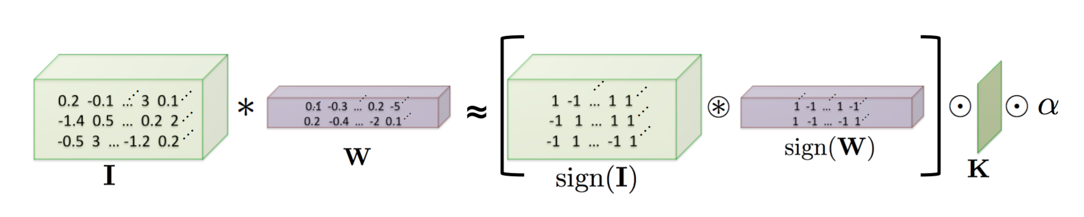
\includegraphics[width=0.8\linewidth]{inc/2_related_work/figure/xnor_operation.png}
    \caption{Convolution with XNOR-Bitcount in XNOR-net from \cite{XnorNet}}
    \label{fig:xnor_operation}
\end{figure}
 
\subsection{8-bit quantization on modern models}
More practically, modern deep models have been showed to work on 8 bits quantization on both weights and activations \cite{TensorRT8bit}. Taking advantage of Nvidia's bulit-in INT8 operations on their GPUs, they developed a CUDA library in TensorRT with an algorithm minimizing loss of information when quantizing trained model without further fine tunning or retraining. Starting with the tensor approximation with quantized tensor:
\begin{equation}
    \begin{aligned}\label{eq:tensorrtop}
    \textbf{Tensor Values}\approx\textbf{FP32 scaling factor}*\textbf{INT8 array}
    \end{aligned}
\end{equation}
 The scaling factor determines the mapping of the quantized level to the original value, for example a scaling factor of $\frac{2.7}{127}$ maps the quantized data 127 to original data 2.7. This is always a trade-off process between range and precision: the larger the scaling is, the larger the range, and the smaller the precision. The scaling process also includes the clipping of data exceeding a pre-defined threshold as seen in \figref{tensorrt_thresold}, and the threshold is in fact the scaling factor times the maximum level of the quantization, which is 127 in INT8 case.
\begin{figure}
    \centering
    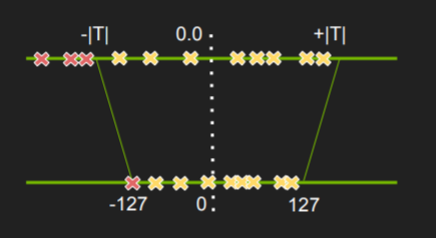
\includegraphics[width=0.5\linewidth]{inc/2_related_work/figure/tensorrt_thresold.png}
    \caption{Information loss is minimized through careful choice of saturation thresold from \cite{TensorRT8bit}}
    \label{fig:tensorrt_thresold}
\end{figure}
\\
Therefore the main challenge here is the choice of the scaling factor.As stated in the work, INT8 model encodes the same information as the original FP32 model, the choosing of the scaling factor is a process of minimizing the loss of information, which can be measured by Kullback-Leibler divergence as the relative entropy or information divergence \eqref{eq:kl_div}. They propose a \textbf{Calibration Dataset} to be run on FP32 format inference, collecting histograms of activations, and then pick thresold that minimize the KL divergence by generating many quantized data distributions with different saturation thresholds. This process is said to take only a few minutes on a desktop workstation. \\ 
\begin{equation}
    \begin{aligned}\label{eq:kl_div}
    \textbf{KL\_Divergence} ( \boldsymbol{P} , \boldsymbol{Q} ) := \textbf{SUM} ( \boldsymbol{P[i]} * log ( \frac{ \boldsymbol{P[i]}}{\boldsymbol{Q[i]}} ) , i)
    \end{aligned}
\end{equation}
The resulting INT8 model achieves no more than \textbf{0.46\%} extra error rate if even not lesser, at the same time speeding up from \textbf{1.62x} to \textbf{3.67x} depending on the inference batch size ( from 1 to 128) on their processor DRIVE PX2, dGPU.
In \autoref{ch:low prec NN} we propose a similar yet simpler scheme to compute the desirable quantization threshold, although our approach involves no calibration after the training, the re-training process is working in low-precision condition and is much slower than train-then-fine-tune scheme in this work. However, we believe that re-training on ultra-low-precision model ( $<$ 8 bits) is still necessary.

\section{Hardware design}
Recently researches related to deep neural network accelerator are blooming rapidly. They typically start off with a core algorithm simplifying the NN model, then combining either micro-architectural optimization such as low-precision arithmetic units or system level optimization involving data compression between the chip and the off-chip memory, delicate buffer design, sparsity-aware zero-skipping operations and so on. \\
We are going to focus on several works that inspire us the most, including modified classic systolic-array style processor operating on a granularity of rows, SIMD (single instruction multiple data) style processor coupled with re-configurable arithmetic unit being able to operate on 1-16 bits respectively.
From these works, we conclude that slashing down memory access counts either from on-chip or off-chip is of upmost importance for chip power efficiency, through further low-bit operation optimization the memory transaction frequency can be furthered improved. 
\subsection{Dataflow optimization: row stationary}
Eyeriss\cite{Eyeriss} analyzes existing accelerator work in a now widely used manner, classifying them into \textit{Weight Stationary}, \textit{Output Stationary}, \textit{No Local Reuse} three dataflows that reuse data differently, and propose a novel processing dataflow coined \textit{Row Stationary}. 
\subsection{Sub-word parallelism arithmetic unit}
\subsection{Bit-level re-configurable arithmetic unit}
\begin{itemize}
    \item \textcolor{purple}{How does related work "relate" to your research question?}
    \item \textcolor{purple}{Does it provide a starting point?}
    \item \textcolor{purple}{Does it provide evidence that you are posing a good research question?}
    \item \textcolor{purple}{Does it provide a different approach to a similar research hypothesis that you can compare to?}
\end{itemize}